\chapter{Configurare}

Pentru a putea fi folosit in cat mai multe moduri, motorul fizic poate fi setat sa ruleze in moduri diferite, iar obiectele sale pot avea mai multe proprietati, descrise mai jos.

\section{Variables}

Variabilele ce pot fi schimbate sunt de 2 tipuri:
\begin{itemize}
    \item variabile de sistem, in fisierul $envrules.h$
    \begin{center}
        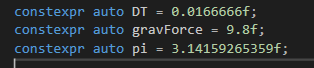
\includegraphics[width=0.3\textwidth]{envrules.png}
    \end{center}
    unde $DT$ reprezinta timpul per frame, $gravForce$ forta gravitationala si $PI$
    \item variabile ale obiectelor
    \begin{itemize}
        \item[-] $gravInvul$, atunci gravitatia nu mai este aplicata obiectelor
        \item[-] $showDirection$
        \begin{center}
        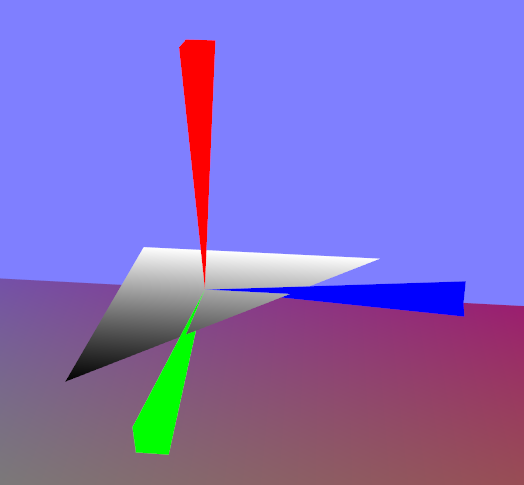
\includegraphics[width=0.3\textwidth]{simple_triangle.png}
        \end{center}
        In cazul in care $showDirection$ este $true$ atunci obiectul va avea 3 axe 
        \begin{itemize}
            \item $Red-Y$
            \item $Green-Z$
            \item $Blue-X$
        \end{itemize} ce reprezenta orientarea obiectului, in caz contrar acestea nu vor aparea.
    \end{itemize}
\end{itemize}


\section{Objects}

 Un obiect fizic este un obiect derivat in $oglVertexObject$ si poate exista in simulator doar daca are un fisier txt in care se regasesc proprietatile si regulile urmatoare:
\begin{itemize}
    \item rotatii dupa o axa oarecare intre $DT1$ si $DT2$ unde $DT2>DT1$. ($DT$\footnote{Delta time, timp scurs de inceperea executiei.})
    \item pozitia x,y,z in world space
    \item factor de elasticitate 
    \item un array de puncte ce reprezinta fiecare varf, aflate oriunde in object space \footnote{puncte in referinta fata de C(0,0,0) unde va fi centrul obiectului.}.
    \item un array de culori ce sunt asignate fiecarui punct
\end{itemize}

De exemplu, pentru urmatorul fisier txt apare un singur triunghi:
\begin{center}
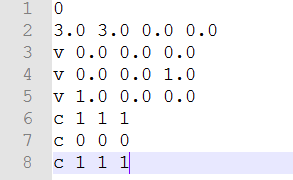
\includegraphics[width=0.3\textwidth]{simple_triangle_txt.png}

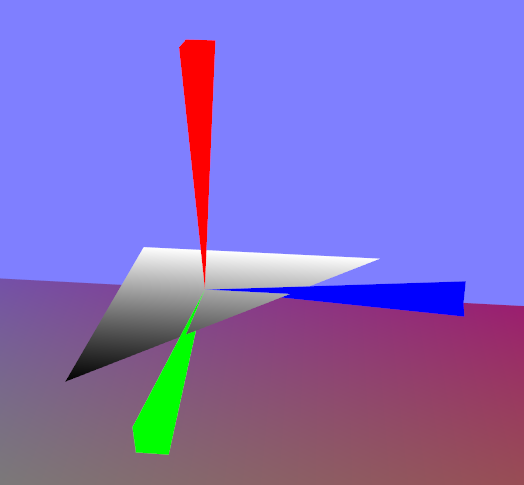
\includegraphics[width=0.3\textwidth]{simple_triangle.png}
\end{center}

Conform fisierului txt, acesta are 0 rotatii, este plasat in punctul $C(3,3,0)$ in world space, are o elasticitate 0, iar varfurile sale reprezinta un triunghi unde varful $V(0,0,1)$ va avea culoarea $RGB(0,0,0)$.

\section{Head}
 
section 

\section{Headless}
 
section 